%\documentclass{article}
%\usepackage[utf8]{inputenc}

%\begin{document}
% Analyse de l'existant >> je ne sais pas qui l'a, je propose mettre
% au moins un exemple du fichier modèle entree (en annexe peut être)   
% avec une mini-description  des params dans un tableau 
% on peut s'entraider pour le faire :)

\section{Déroulement du projet} 

\subsection{Planification}

Le développement de l'interface web pour l'utilisation du 
logiciel dédié au calcul de Maximum de vraisemblance \textit{bppml} suivra les
 étapes suivantes:

\begin{itemize}
	\item Installation et test de fonctionnement de pbbsuite: la suite logicielle est installée en local sur nos machines. 
	Parmi les douze logiciels qui en font partie, spécifiquement   \textit{bppml} a été choisi par le demandeur de la prestation comme cible 
	du développement web du présent travail. Des exemples de fichiers de configuration (contenant \textit{a minima} les éléments: alignement, arbre(s), modèle(s)) 
	ont été mis a notre disposition  
	afin de tester plusieurs scenarios possibles, du plus simple, en passant par les cas les plus fréquents "standard", 
	jusqu'aux modèles plus exigeantes comptant d'avantage de paramètres. Pendant cette étape nous aurons l'opportunité d'explorer
	 la modélisation des processus évolutifs en phylogénie.
	
	\item Développement d'une application en locale: le framework python FLASK et des librairies npm
	(le gestionnaire de paquets officiel de Node.js) 
	ont été choisis en raison du bon rapport entre flexibilité et stabilité, 
	ayant une ample gamme de librairies disponibles pour un développement rapide et au même temps efficace, 
	ce qui est convenable en raison des contraintes de temps du projet.

	On produira un premier prototype  \textit{bpp-web}, acceptant en entrée un modèle ayant les paramètres minimaux requis. 
	Cette application intermédiaire sera rapidement enrichie pour offrir à l'utilisateur de \textit{bppml} la totalité des possibles affectations 
	des variables (plusieurs arbres, plusieurs modèles).
	Ceci sera réalisé en trois phases parallèles:
	\begin{enumerate}
		\item Développement de l'interface entrée qui permettra un usage intuitif de la part du utilisateur. 
		Un script .js capture les variables insérées par l'utilisateur. 
		\item Scripting pour la transmission des variables depuis celles capturées par .js en passant par le langage 
		python (Flask) jusqu'un fichier .txt qui est donné en entrée au logiciel \textit{bppml}.
		\item Scripting pour la capture soit des résultats, soit des messages d'erreur (stderr) et transmission à travers 
		le framework Flask vers le client, et visualisation de l'arbre obtenu \textit{in situ}. 
	\end{enumerate}
	
	La possibilité de boucler des résultats vers l'entrée client sera étudiée.
	 
	\item La Version définitive de \textit{bpp-web} reposera sur le même framework développé
	à l'étape précédente, ce qui sera réalisé en deux pas simultanés:
	\begin{itemize}
		\item la mise en place et déploiement de l'interface web sur un Serveur Linux.
		\item l'exécution des derniers tests et correction d'éventuels erreurs.
	\end{itemize}
	
	Les délais pour chacune des étapes du projet sont visualisés dans la figure~\ref{planning}.
	\begin{figure}[ht!]
		\caption{\label{planning} Chronologie de l'exécution du projet}
		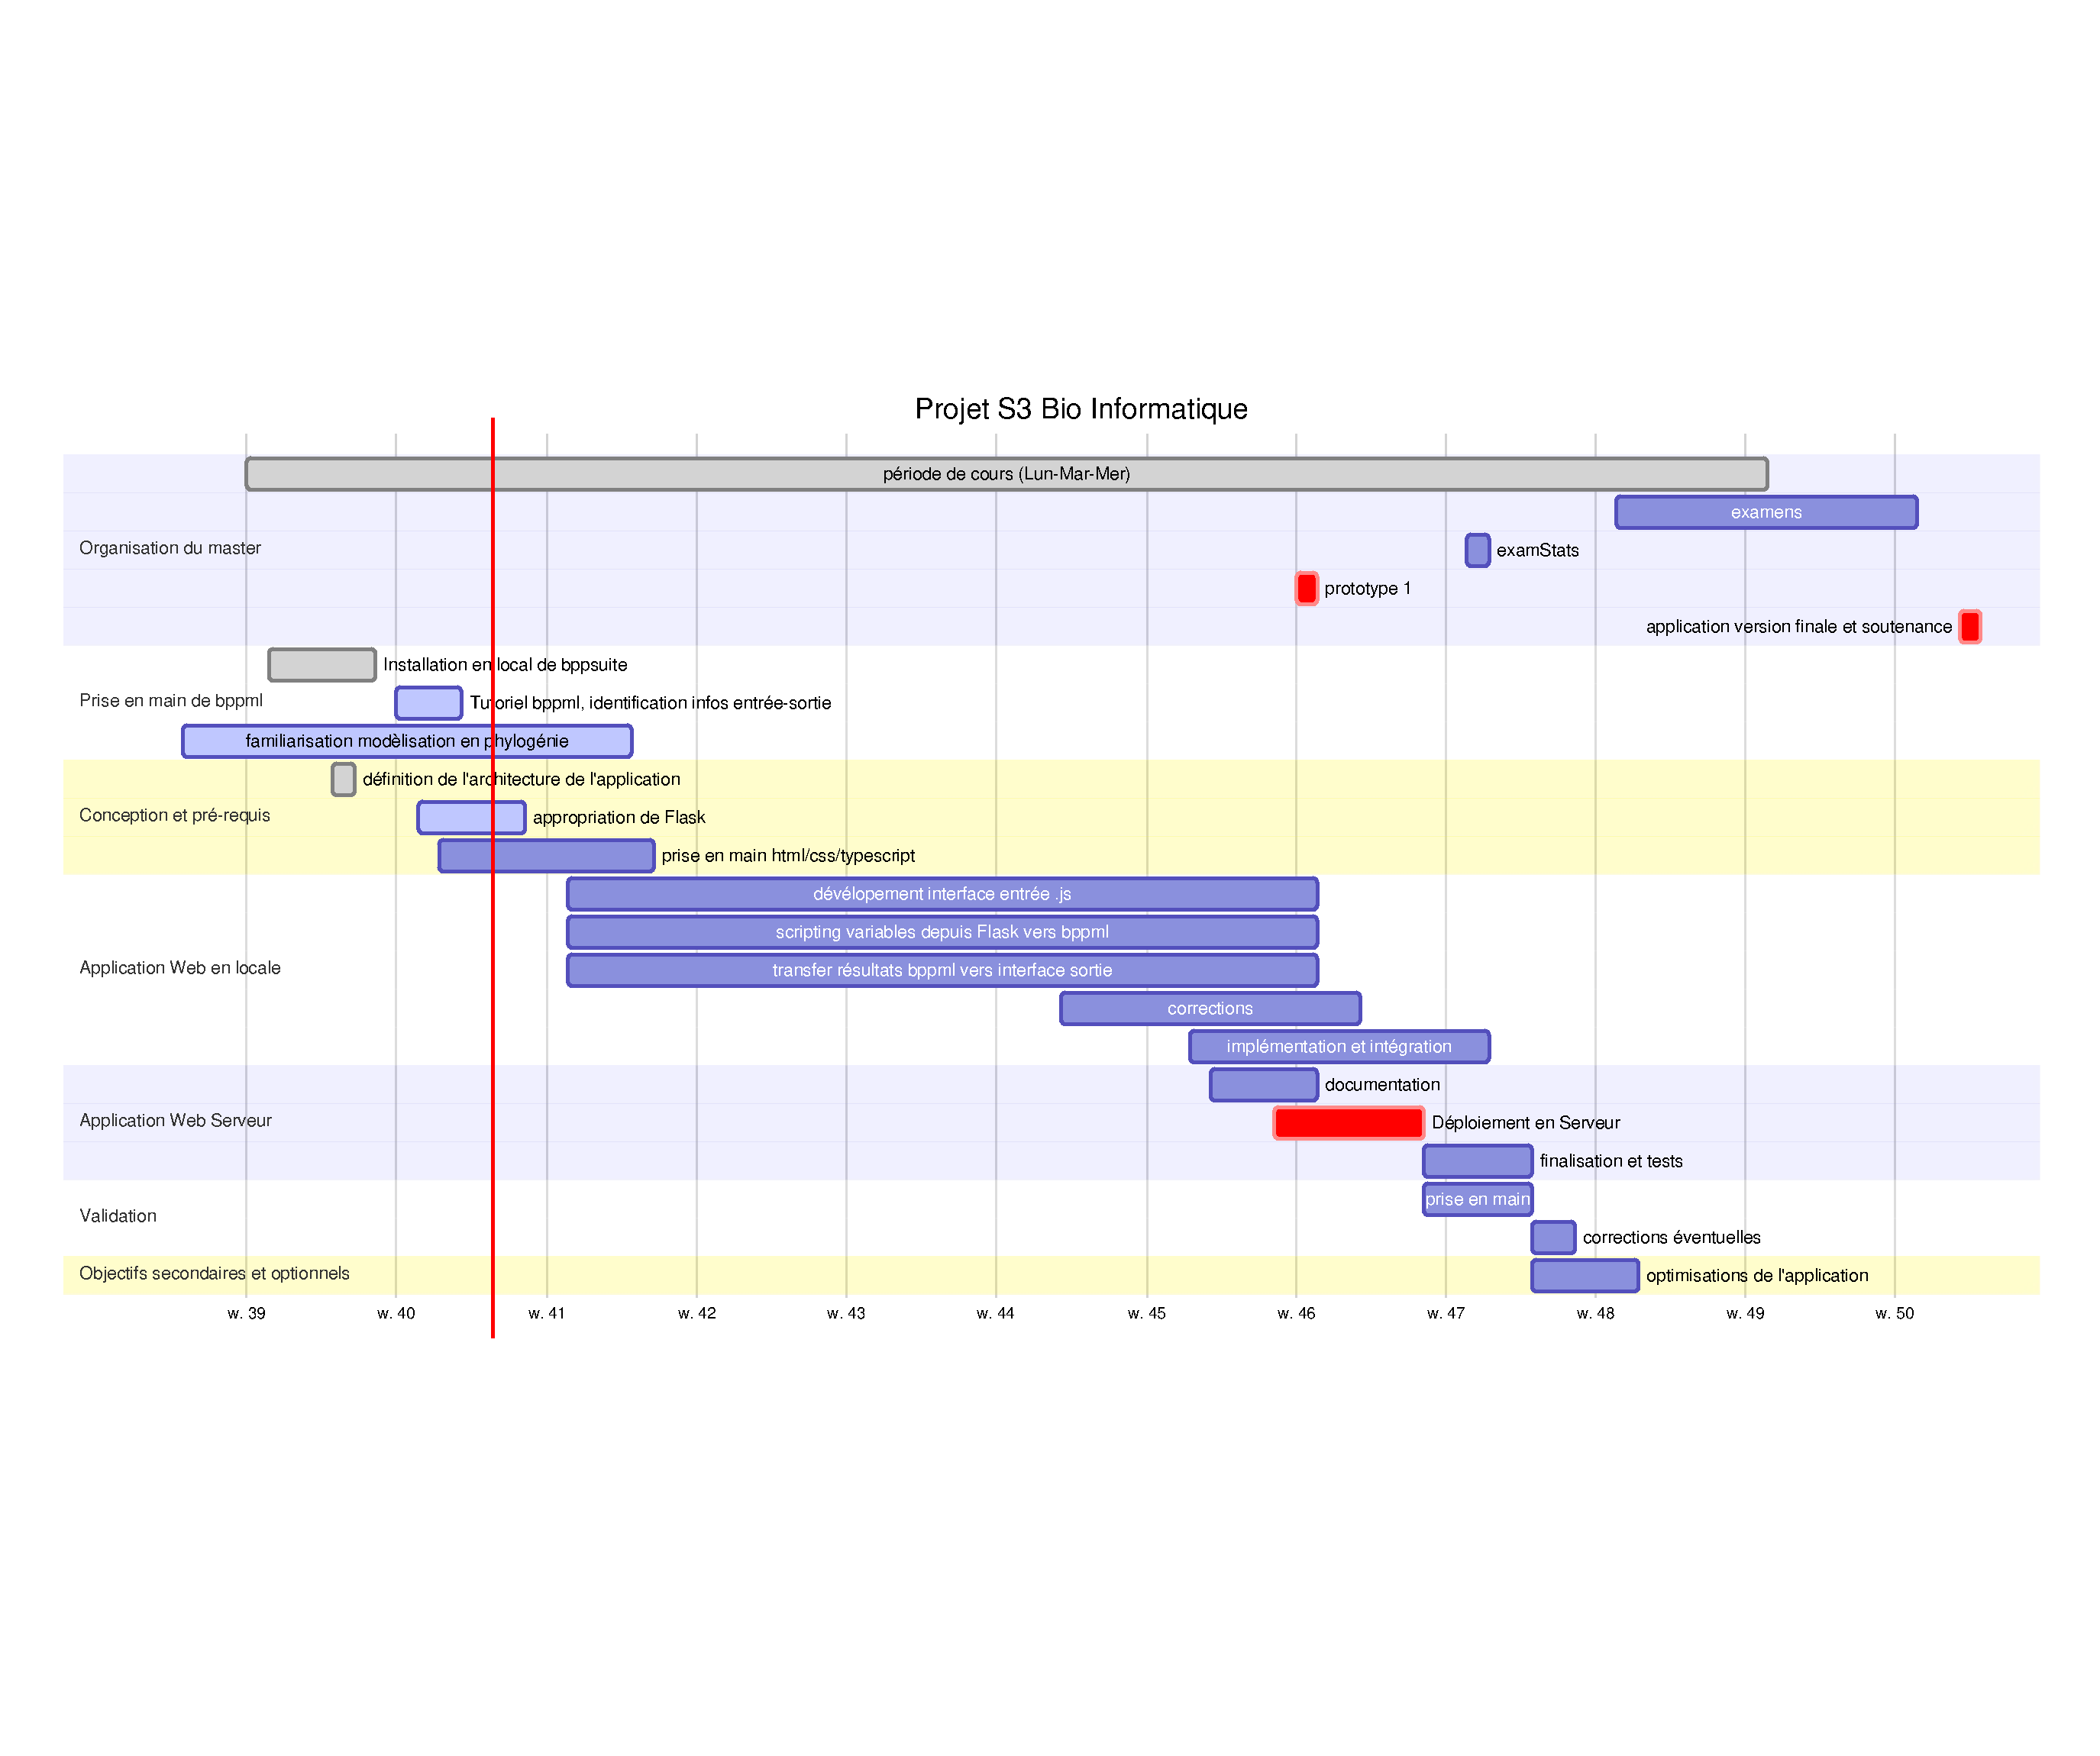
\includegraphics[trim={1.5cm 8cm 2cm 8cm},clip,width=\textwidth]{fig/mermaid1.pdf}
	\end{figure}
	
	La prestation sera orientée vers la possibilité de faire évoluer le code (par exemple, par d'autres équipes invitées) 
	afin de couvrir progressivement d'avantage de logiciels faisant partie de \textit{bppsuite} et \textit{Bio++}.
\end{itemize}


\subsection{Plan d'assurance qualité}
 Pour contrôler la qualité du logiciel, à chaque test effectué la sortie sera  
 évaluée sous critères de cohérence, complétude (aucun fichier de sortie omis ou délaissé)
 et structure. Sur des modèles plus complexes, l'aval des sorties par l'expert du logiciel \textit{bppml} sera nécessaire.

De plus, le projet sera conduit
sous un modèle de travail collaboratif efficace,
préconisant développement itératif des fonctionnalités de l'interface,
avec l'ajout progressif de fonctions de plus en plus avancées.
La coordination étroite des membres du projet
assurera la bonne avancée en parallèle de l'implémentation des différentes composantes.
Le respect de standards de programmation rigoureux
garantira aussi un développement robuste et efficace face aux difficultés potentielles,
et un socle solide pour une extension future au delà du projet.

Des dispositifs de l'université,
dont des salles de travail disponibles aux étudiants du master bioinformatique,
et des systèmes de visioconférence,
pourraient aider à pallier à la contrainte du travail à distance.

 
\subsection{Documentation} 
La documentation sera apportée en totalité dans un dépôt GitHub.

	
\subsection{Responsabilités}
\subsubsection{Maîtrise d'ouvrage}
L'équipe \textit{Bio++} development team, représentée par M. Laurent Guéguen est le
 demandeur du présent travail. Les délais données correspondent a ceux de la matière 
 Projet du M2 bio-info, ayant pour dates clés les suivantes:
\begin{itemize}
	\item 25/09 : description des besoins par le maître d'ouvrage.
	\item 30/09 : apport des exemples et Tutoriel par le maître d'ouvrage.
	\item 09/10 : rendu du cahier des charges 
	\item 17/12 : délivrable et soutenance 
\end{itemize}
Il n'y a pas de budget officiel institutionnel consacré à ce projet. 

\subsubsection{Maîtrise d'oeuvre}

Les trois branches simultanées de développement sont attribuées comme suit:

\begin{itemize}
	\item Hadrien : interface entrée client, capture des variables.
	\item Konstantinn : conduction des variables depuis.js vers .py et \textit{bppml}.
	\item Johanna : interface sortie client, visualisation des résultats.
\end{itemize}


Le tuteur pédagogique est M. Guillaume Launay.

%\end{document}
